%\documentclass[10pt]{article}
\documentclass[10pt]{tufte-handout}


\usepackage[utf8]{inputenc}
\renewcommand*{\familydefault}{\sfdefault}

\usepackage{graphicx}      
\usepackage{hyperref}       
\usepackage{amsmath, amssymb}

%\usepackage{fullpage}

\usepackage{tikz}


\title{A probabilistic user model for information retrieval}
\author{A1, A2}
\date{}

\begin{document}
\maketitle
\begin{abstract}
 A general level probabilistic user model for information retrieval is derived from the basic problem definition. The model is shown to work on various example scenarios and extensions such as new modes of feedback are discussed.
\end{abstract}

\section{Introduction}

\section{Definition}
\subsection{Problem}
An information retrieval system needs to solve the problem of incomplete knowledge of user's information need. Some key components must be defined in order to realize any such system.

First component is a known collection $C$ of retrieval items. Each item in the collection $d_i \in C$ must have a quantification: Call such quantification the feature representation $x_i\in \mathcal X$ with some [metric] space $\mathcal X$. 

For example, a piece of music can be described by the artist, title and record labels, each represented as value 1 of a corresponding binary variable in the joint space of all possible artist, title and record names. 

Second component is the representation of information need. This can be formalized by equating the information need $\theta$ with a distribution in the feature space. For example with some parametric distribution family we would set $P(event\ A) = \int_A f_\theta (x) dx$ where the parameters define the 

Last component is the representation of relevance, expressed as a variable $r\in \mathbb R$, often defined only on the unit interval. A typical choice interprets the value 0 as 'not relevant' and 1 as 'relevant'. Binary choice is often made, with the downside of losing e.g. interpretation of a value 0.5 as 'irrelevant', and so forth.

\subsection{Solution}
The three components are now connected to make the dependency graph of a solution. Note that the minimal solution graph has at least two edges, as any less would render a component independent of the other two and our problem definition redundant.

\begin{marginfigure}%
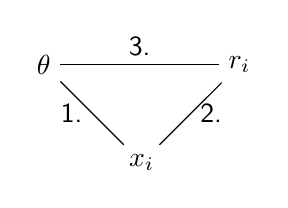
\begin{tikzpicture}[node distance=5em]
  \node[] (doc) {$x_i$};
  \node[above right of=doc] (rel) {$r_i$};
  \node[above left of=doc] (theta) {$\theta$};

  \draw[] (theta) -- node [left] {1.} (doc);
  \draw[] (doc) -- node [right] {2.} (rel);
  \draw[] (theta) -- node [above] {3.} (rel);
\end{tikzpicture}
\caption{Complete graph.}
\label{fig:graph1}
\end{marginfigure}

\begin{marginfigure}%
\begin{tikzpicture}[node distance=5em]
  \node[] (doc) {$x_i$};
  \node[above right of=doc] (rel) {$r_i$};
  \node[above left of=doc] (theta) {$\theta$};

  \draw[] (doc) -- (rel);
  \draw[] (theta) -- (rel);
\end{tikzpicture}
\caption{Solution graph.}
\label{fig:graph2}
\end{marginfigure}

The complete graph (Figure~\ref{fig:graph1}) is not useful: consider
the two possible cases of effect. If the user's information need would
affect the feature representation, the change of a user would violate
the first assumption of a known collection. Vice versa the feature
representation should not affect what the user is looking for, but
affect only the system's internal operation. Therefore the solution
has two edges, connecting the information need with the items through
relevance (Figure~\ref{fig:graph2}).

Having fixed the dependency structure of the three components, the
next step is to argue the direction of the effects ...

\begin{marginfigure}%
\begin{tikzpicture}[node distance=5em]
  \node (theta) {$\theta$};
  \node[right of=theta] (rel) {$r_i$};
  
  \draw[->] (theta) -- (rel);
\end{tikzpicture}

\noindent\begin{tikzpicture}[node distance=5em]
  \node (theta) {$\theta$};
  \node[right of=theta] (rel) {$r_i$};
  
  \draw[<-] (theta) -- (rel);
\end{tikzpicture}
\caption{Possible effect directions between information need and
  relevance.}
\label{fig:graph3}
\end{marginfigure}

\begin{marginfigure}%
\begin{tikzpicture}[node distance=5em]
  \node (doc) {$x_i$};
  \node[right of=theta] (rel) {$r_i$};
  
  \draw[->] (doc) -- (rel);
\end{tikzpicture}

\noindent\begin{tikzpicture}[node distance=5em]
  \node (doc) {$x_i$};
  \node[right of=doc] (rel) {$r_i$};
  
  \draw[<-] (doc) -- (rel);
\end{tikzpicture}
\caption{Possible effect directions between documents and
  relevance.}
\label{fig:graph4}
\end{marginfigure}

The final solution then is ...

\begin{marginfigure}%
\noindent\begin{tikzpicture}[node distance=5em]
 \node[] (doc) {$x_i$};
  \node[above right of=doc] (rel) {$r_i$};
  \node[above left of=doc] (theta) {$\theta$};

  \draw[->] (doc) -- (rel);
  \draw[->] (theta) -- (rel);
\end{tikzpicture}
\caption{Final solution.}
\label{fig:graph5}
\end{marginfigure}


\section{Properties}

In this section we have interpretation of higher level quantities. Session, information drift, precision-recall, feedback.

Session:

Precision-recall:

Feedback: implicit, explicit, pseudo


\section{Examples}

\section{Discussion}


\end{document}  
